\section{Theory}

In solving the linking problem, one must find a way to compare different
documents based on their linkability with a newly added documents.
Computationally, this can be done by creating document descriptors -- vectors
that the describe the features of a document in some way. Given the Starfish
domain, this can be done in a tag-based and text-based approach towards
creating document descriptors. This section will elaborate the background of
the descriptor-based approach. 

\subsection{Text-based descriptors: bag of words and TF-IDF}
One way of capturing the semantic similarity of two text document is by
comparing the TF-IDF values of their contents. If two documents cover the same
subject(s), they are likely to contain similar keywords. To capture this
similarity, the documents can be transformed into a list of all words that are
present within that text. This is called a bag-of-words representation. Instead
of counting the frequency of each word within a document, the more
sophisticated Term Frequency-Inversed Document Frequency value can be used.
TF-IDF is a statistic that reflects the importance of a word in a document
within a corpus and can be calculated as follows:

\begin{align}
\textrm{tf}(t,d) = 0.5 + \frac{0.5 \times {f}(t, d)}{\max\{{f}(w, d):w \in d\}}\\
\textrm{idf}(t, D) =  \log \frac{N}{|\{d \in D: t \in d\}|}\\
\textrm{tfidf}(t,d,D) = \textrm{tf}(t,d) \times \textrm{idf}(t, D)
\end{align}

The TF-IDF induces a trade-off between the term frequency, the number of times
a word appears in a document, and the inverse document frequency, the inverse
of how often a word is used in the entire corpus. Words such as `and', `or',
and `of' will have a high term frequency within a document. However, their
inversed document frequency will be very low, since they occur very often
within the entire corpus. Infrequent words such as `clicker' are less likely to
occur within a corpus, so if they do occur often within one particular document
the TF-IDF value will be high. 

\subsection{K-Nearest Neighbor}
After creating the document descriptors as described in the previous section
all document lay in a specific vector space. For each of this vectors we
can compute a distance using a specific distance measure. The $K$-Nearest
Neighbor algorithms selects the $K$ document descriptors that have the lowest
distance. In other words the $K$ vectors that are most similar in the given
vector space. See algorithm~\ref{algo:knn} for pseudocode of the $K$-Nearest
Neighbir algorithm.

\begin{algorithm}                      
  \caption{$K$-Nearest Neighbor}      
  \label{algo:knn}
  \begin{algorithmic}

    \STATE docs $=$ Vector document descriptors.
    \STATE dist $=$ Vector document distance metric.
    \STATE d $=$ Document to find neighbors of.
    \STATE $\delta$ = []
    \FOR{doc $\in$ docs} 
      \STATE $\delta \Leftarrow$ (doc, dist(d, doc))
      \COMMENT{Compute distance with every document}
    \ENDFOR
    \STATE sorted $=$ sort(delta)
    \COMMENT{Sort from lowest to highest distance}
    \RETURN sorted$[0\ldots K]$
    \COMMENT{Return $K$ first documents}
  \end{algorithmic}
\end{algorithm}

\subsubsection{Distance Metric}
As discussed before the $K$-Nearest Neighbor algorithm uses a distance metric
to compute the distance between two document descriptors in a given vector
space. A distance metric or simply called the distance is a function $d$ that 
maps two documents descriptors $X$ and $Y$ to the real numbers (\ref{distmap}).
\begin{align}
  d : X \times Y \mapsto \mathbb{R} \label{distmap}
\end{align}
This function $d$ at least satisfies the following conditions for the documents
$X$, $Y$ and $Z$.
\begin{align*}
  1.\ \ \ & d(X,Y) \geq 0 \\
  2.\ \ \ & d(X,Y) = 0\  \text{if and only if $X=Y$} \\
  3.\ \ \ & d(X,Y) = d(Y,X) \\
  4.\ \ \ & d(X,Z) \leq d(X,Y) + d(Y,Z)
\end{align*}

A set of distance metrics is discussed in the following paragraphs. Each are
discussed for a documents with documents descriptor  $q = [q_1, q_2, \ldots,
q_n]^T$ and $p = [p_1, p_2, \ldots p_n]^T$.


\paragraph{Euclidean distance}
The euclidean distance metric is a generalization of the pythagorean metric to
higher dimensions. The euclidean distance is the ruler distance or in other 
words the distance between the two heads of each vector.

\begin{align*}
  d_{\text{euclid}}(q,p) &= \sqrt{(q_1 - p_1)^2 + (q_2 - p_2)^2 + \cdots + (q_n - p_n)^2}  \\
                         &= \sqrt{\sum_{i=1}^n (q_i - p_i)^2} \\
                         &= \sqrt {(q-p) \cdot (q-p)} \\
                         &= || q - p ||
\end{align*}
This shows that the euclidean distance is the norm of the vector $p-q$ or 
$q-p$ (as $d(q,p) = d(p,q)$). This makes sense as the euclidean distance
is the distance between the two vectors. An illustration of this is given in
figure~\ref{fig:euclid}

\begin{figure}[h!]
 \center
 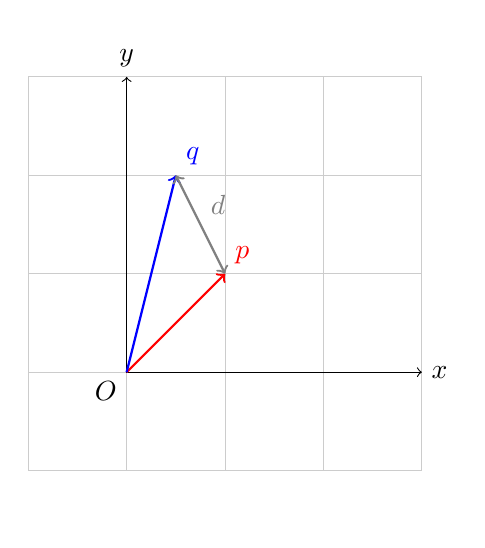
\begin{tikzpicture}[scale=2.5]
   \fill [white] (-.5,1.75) rectangle (1.5, -.75);
   \draw[step=0.5,gray!40,thin] (-.5,-.5) grid (1.5,1.5);

   % Draw axes
   \draw [<->] (0,1.5) node (yaxis) [above] {$y$}
     |- (1.5,0) node (xaxis) [right] {$x$};
 
   \draw [->, thick, red] (0,0) -- (0.5,0.5) node [above right] {$p$};
   \draw [->, thick, blue] (0,0) -- (0.25,1.0) node [above right] {$q$};

   \draw [<->, thick, gray] (0.5,0.5) -- (0.375, 0.75) node [above right] {$d$} -- (0.25,1.0);
 
   % \draw [->] (0.4, 0) arc (0:20:0.4) node [above right,inner sep=0pt] {\small{$\theta$}} arc (20:45:0.4);
 
   \draw (0,0) node [below left] {$O$};
\end{tikzpicture}

 \caption{The euclidean distance $d$ between two document descriptors $p$ and $q$.}
 \label{fig:euclid}
\end{figure}

\paragraph{Cosine distance} The cosine distance measures the cosine of the
angle $\varphi$ between two document descriptors. The intuition of this metric
is that a document `word$_1$ word$_2$' and `word$_1$ word$_1$ word$_2$
word$_2$' probably are very similar as only the word frequencies differ.
However, the euclidean distance does compute a distance $> 0$. The cosine
distance computes the angle between two documents. This is shown visualy in
figure~\ref{fig:cosine}. In this example the descriptors would point in the
exact same direction only the second descriptor is longer.  This results in a
cosine of zero, which means an exact match. The values in the vectors will
never take a value $< 0$ because a word can not occur less then zero times.
Because of this the values of the cosine of the angle between two descriptors
will range between $0$ and $1$. Where 0 means no match at all and 1 is an exact
match. Therefore the cosine distance is defined as:
\begin{align*}
  d_\textrm{cos}(q,p) = |\cos(\varphi) - 1|
\end{align*}
where $\varphi$ is the angle between $q$ and $p$. Given that $q \cdot p = ||q||
\,||p|| \cos(\varphi)$ we can easily compute the $\cos(\varphi)$. This results
in the definition of the cosine distance metric in equation~\ref{eq:cos}. It is
very efficient to compute the cosine distance on sparse vectors as only the
non-zero values are important for the computation.

\begin{align}
  d_\textrm{cos}(q,p) = \left| \frac{q \cdot p}{||q||\,||p||} - 1\right| \label{eq:cos}
\end{align}

\begin{figure}[h!]
 \center
 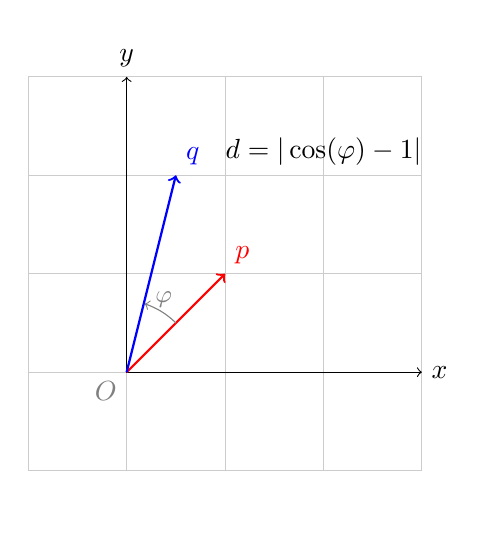
\begin{tikzpicture}[scale=2.5]
   \fill [white] (-.5,1.75) rectangle (1.5, -.75);
   \draw[step=0.5,gray!40,thin] (-.5,-.5) grid (1.5,1.5);

   % Draw axes
   \draw [<->] (0,1.5) node (yaxis) [above] {$y$}
     |- (1.5,0) node (xaxis) [right] {$x$};
 
   \draw [->, thick, red] (0,0) -- (0.5,0.5) node [above right] {$p$};
   \draw [->, thick, blue] (0,0) -- (0.25,1.0) node [above right] {$q$};

   \draw [->, gray] (0.25, 0.25) arc (45:64:0.4) node [above right,inner sep=0pt] {\small{$\varphi$}} arc (64:72:0.4);

   \draw (1,1) node [above] {$d = |\cos(\varphi)-1|$};
 
   \draw [gray] (0,0) node [below left] {$O$};
\end{tikzpicture}

 \caption{The cosine distance $d$ between two document descriptors $p$ and $q$.}
 \label{fig:cosine}
\end{figure}

\paragraph{Bhattacharyya distance} The feature vectors used to represent documents can
also be seen as unordered histrograms. A way to compare histrograms is the
Bhattacharyya distance metric. The Bhattacharyya metric is used to compute
the similarity of two discrete or continuous probability distributions. The 
metric ranges from 0 tot 1 where 0 is a perfect match. The Bhattacharyya 
distance metric is defined as:
\begin{align}
  d_B (q,p) = \sqrt{1 - \frac{1}{\sqrt{\overline{q}\,\overline{p}n^2}}\sum_{i=1}^n \sqrt{q_ip_i}}
\end{align}
where $\overline{q} = \frac{1}{n}\sum_{j=1}^n q_j$ and $n$ the number of
elements in each of the vectors.

\paragraph{Intersection} Another histrogram similarity metric is the histogram
intersection. The histogram intersection \citep{swain1991color} was originaly
introduced in the computer vision field and is defined in as shown in
equation~\ref{eq:intersection}
\begin{align}
  d_\textrm{int}(q,p) = \sum_{i=1}^n \min(q_i, p_i) \label{eq:intersection}
\end{align}
In the computer vision domain this results in the number of pixels that have
the same color. For the document descriptors used in this case this comes
down to the weights the two documents have in common. In other words when
two documents that have high weights for the same words the total will be
higher then when two documents have hight weights for different words. This
measure does not satisfy the four conditions for a distance metric, however
it may still be useful in the document similarity domain.

\paragraph{Cross-correlation} Finally a method often used to compute the
similarity between histograms is the cross-correlation. 
\todo[inline]{Show that correlations is equivalent to cosine distance}

